\documentclass[xcolor=dvipsnames]{beamer} % dvipsnames gives more built-in colors
\usepackage{graphicx}
\usetheme{Luebeck}
\useoutertheme{infolines} % Alternatively: miniframes, infolines, split
\useinnertheme{circles}
\usepackage{subcaption}
\usepackage{listings}
\usepackage{tikz,tikz-3dplot}
\usetikzlibrary{calc,arrows}
\usepackage{xcolor}
\lstset{
	basicstyle=\ttfamily\tiny,
	basewidth=0.65em,
	commentstyle=\ttfamily,
	tabsize=2,
	keywordstyle=\bfseries\sffamily,
	showstringspaces=false,
	numberstyle=\tiny,
	numbersep=2.5pt,
	keywordstyle=\bfseries\ttfamily,
	breaklines=true
}
\lstnewenvironment{pseudoc}{\lstset{frame=lines,mathescape=true, language = C++, basicstyle=\ttfamily\small, basewidth=0.55em}}{}

\definecolor{UBCblue}{rgb}{0.04706, 0.13725, 0.26667} % UBC Blue (primary)

\usecolortheme[named=MidnightBlue]{structure}
%\usecolortheme[named=Mahogany]{structure} % Sample dvipsnames color

\title[Valutazione del Contatto Pneumatico/Strada]{Valutazione Real-Time del Contatto Pneumatico/Strada con Algoritmi Dedicati}
\date{}

\usepackage{fontspec}
\defaultfontfeatures{Mapping=tex-text}
\setromanfont[Ligatures={Common}]{Adobe Caslon Pro}
\usefonttheme{serif}

\begin{document}

\begin{frame}[fragile]
	\begin{center}
		\huge{\textbf{Intersezione trà alberi di tipo AABB}}
	\end{center}
\end{frame}

\begin{frame}[fragile]
	\Large{\textbf{Intersezione trà alberi di tipo AABB}}
	\normalsize
	\\[0.2cm]
	Volendo intersecare due semplici AABB, quali:
	\begin{equation*}
	\begin{split}
	A = \left[ \texttt{A.minX}, \texttt{A.maxX},  \texttt{A.minY}, \texttt{A.maxY} \right]\\
	B = \left[ \texttt{B.minX}, \texttt{B.maxX},  \texttt{B.minY}, \texttt{B.maxY} \right]
	\end{split}
	\end{equation*}
	verrà usata la seguente funzione:
	\vspace{.8em}
\begin{pseudoc}
function intersect(A,B) {
    return (A.minX <= B.maxX && A.maxX >= B.minX) &&
    (A.minY <= B.maxY && A.maxY >= B.minY)
}
\end{pseudoc}
\end{frame}

\begin{frame}[fragile]
	\begin{center}
		\huge{\textbf{Intersezione trà entità geometriche}}
	\end{center}
\end{frame}

\begin{frame}[fragile]
	\Large{\textbf{Intersezione segmento-punto}}
	\normalsize
	\\[0.2cm]
	Dato un punto $P = (x_p, y_p)$ e un segmento definito dai punti $A = (x_A, y_B)$ e $B = (x_B, y_B)$.
	\begin{figure}[h!]
		\centering
		\begin{tikzpicture}
		\def\r{2};
		\coordinate (P) at (0.3,0.7);
		\coordinate (A) at (-2.0,0.0);
		\coordinate (B) at (+2.0,0.0);
		\draw[fill] (A) circle [radius=1pt] node[above] {$A$};
		\draw[fill] (B) circle [radius=1pt] node[above] {$B$};
		\draw[fill] (P) circle [radius=1pt] node[above] {$P$};
		\draw[thick](A) -- (B);
		\end{tikzpicture}
	\end{figure}
	\noindent
	Per determinare se il punto $P$ è interno al segmento gli \textit{step} sono:
	\begin{enumerate}
		\item creazione di un vettore $\vec{AB}$ e di un vettore $\vec{AP}$;
		\item calcolo del prodotto vettoriale  $\vec{AB} \times  \vec{PA}$, se il modulo del vettore risultante è nullo allora il punto $P$ appartiene al segmento considerato;
		\item calcolo del prodotto scalare tra $\vec{AB}$ e $\vec{AP}$, se è nullo allora $P \equiv A$, se è pari al modulo di $\vec{AB}$ allora il $P \equiv B$, se è compreso tra 0 il modulo di $\vec{AB}$, allora il punto $P$ giace all'interno del segmento considerato.
	\end{enumerate}
\end{frame}

\begin{frame}[fragile]
	\Large{\textbf{Intersezione punto-cerchio}}
	\normalsize
	\\[0.2cm]
	Data una circonferenza con centro $C = (x_c, y_c)$ e raggio $r$, il problema consiste nel trovare se un generico punto $P = (x_p, y_p)$ è all'interno, all'esterno o corrispondente alla circonferenza.
	\begin{figure}[h]
		\centering
		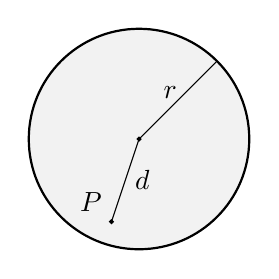
\begin{tikzpicture}[scale=0.7]
		\def\r{2};
		\coordinate (C) at (0,0) node[above left] {$C$};
		\draw[thick, fill=gray!10](C) circle (\r);
		\coordinate (P) at (-0.5,-1.5);
		\draw[fill] (C) circle [radius=1pt];
		\draw[fill] (P) circle [radius=1pt];
		\draw(C) -- (P)  node[above left] {$P$} node[pos=0.5, right] {$d$};
		\draw(C) -- ({sqrt(\r)},{sqrt(\r)}) node[pos=0.4, above] {$r$};
		\end{tikzpicture}
	\end{figure}
	La soluzione al problema è semplice: la distanza tra il centro della circonferenza $C$ e il punto $P$ è data dal teorema di Pitagora, ovvero:
	\begin{equation*}
	d=\sqrt{(x_p-x_c)^2 + (y_p-y_c)^2}
	\end{equation*}
\end{frame}

\begin{frame}[fragile]
	\Large{\textbf{Intersezione piano-piano}}
	\normalsize
	\\[0.2cm]
	\begin{figure}
		\centering
		\tdplotsetmaincoords{70}{110}
		\begin{tikzpicture}[tdplot_main_coords,font=\sffamily, scale= 0.7]
		\draw[-latex] (0,0,0) -- (4,0,0) node[left] {$x$};
		\draw[-latex] (0,0,0) -- (0,4,0) node[below] {$y$};
		\draw[-latex] (0,0,0) -- (0,0,4) node[left] {$z$};
		\tdplotsetrotatedcoords{45}{0}{0}
		\begin{scope}[tdplot_rotated_coords]
		\draw[fill=gray!10,opacity=0.6] (-3,0,-3) -- (-3,0,3) -- (3,0,3) -- (3,0,-3) -- cycle;
		\end{scope}
		\tdplotsetrotatedcoords{90}{45}{0}
		\begin{scope}[tdplot_rotated_coords]
		\draw[fill=gray!10,opacity=0.5] (-3,-3,0) -- (-3,3,0) -- (3,3,0) -- (3,-3,0) -- cycle;
		\draw[thick](-3,{3/sqrt(2)},0) coordinate(x) --(3,{-3/sqrt(2)},0);
		\end{scope}
		\node[anchor=south east,align=center] (line) at (3,-1.5,3.5) {$L$};
		\draw[-latex] (line) to[out=0,in=135] (x);
		\end{tikzpicture}
	\end{figure}
	\begin{equation*}
		L(s) = \frac{(d_2\vec{n}_1 - d_1\vec{n}_2) \times \vec{u}}{|\vec{u}|^2}+s\vec{u}
	\end{equation*}
\end{frame}

\begin{frame}[fragile]
	\Large{\textbf{Intersezione piano-segmento e piano-raggio}}
	\normalsize
	\\[0.2cm]
	\begin{figure}
		\centering
		\tdplotsetmaincoords{70}{110}
		\begin{tikzpicture}[tdplot_main_coords]
		\draw[-latex] (0,0,0) -- (4,0,0) node[left] {$x$};
		\draw[-latex] (0,0,0) -- (0,4,0) node[below] {$y$};
		\draw[-latex] (0,0,0) -- (0,0,4) node[left] {$z$};
		
		\draw[fill=gray!10,opacity=0.5] (-3,-3,0) -- (-3,3,0) -- (3,3,0) -- (3,-3,0) -- cycle;
		\draw[-stealth,thick] (0,-0.75,3.25) node[above] {$P_0$} -- (0,1.25,1.25) node[above right] {$P_1$};
		\draw (0,-0.5,2.25) node[below left] {$\vec{w}$};
		\draw (0,0.25,2.25) node[above right] {$\vec{u}$};
		\draw[-stealth,thick] (0,0,0) -- (0,-0.75,3.25);
		\draw[dashed] (0,1.25,1.25) -- (0,2.5,0);
		\draw[fill] (0,2.5,0) circle [radius=1pt];
		\draw (0,2.5,0) node[below left] {$P(t_I)$};
		\draw (0,2,0.5) node[right] {$P(t)$};
		\draw[fill] (0,2,.5) circle [radius=1pt];
		\draw[-stealth,thick] (1,-2,0) -- (1,-2,2) node[left] {$\vec{n}$};
		\end{tikzpicture}
	\end{figure}
	\begin{equation*}
	\vec{n} \cdot (\vec{w}+t\vec{u}) = 0
	\qquad
	t_I = -\frac{\vec{n}\cdot\vec{w}}{\vec{n}\cdot\vec{u}}
	\end{equation*}
\end{frame}

\begin{frame}[fragile]
	\Large{\textbf{Intersezione raggio-triangolo}}
	\normalsize
	\\[0.2cm]
\begin{figure}[htbp]
	\centering
	\hfill
	\begin{subfigure}[t]{.45\linewidth}
		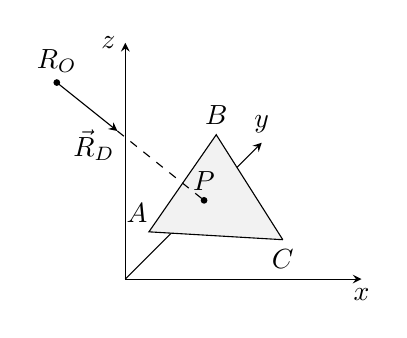
\begin{tikzpicture}
		\coordinate (O) at (0,0,0);
		\def\axisl{3}
		\draw[-stealth] (O) -- (\axisl,0,0) node[below]{$x$};
		\draw[-stealth] (O) -- ({sqrt(\axisl)},{sqrt(\axisl)},0) node[above]{$y$};
		\draw[-stealth] (O) -- (0,\axisl,0) node[left]{$z$};
		\coordinate [label=below:$C$] (V1) at ({\axisl/1.5},0.5,0);
		\coordinate [label=above:$B$] (V2) at ({sqrt(\axisl)/1.5},{3.3/1.8},0);
		\coordinate [label={[shift={(-0.15,0)}]$A$}] (V3) at (0.3,0.6,0);
		\draw[fill=gray!10] (V1) -- (V2) -- (V3) -- (V1);
		
		\def\xp{1};
		\def\yp{1};
		\def\xd{-1};
		\def\yd{0.8};
		\def\mag{1.7};
		\coordinate [label=above:$P$] (P) at (\xp,\yp);
		\coordinate [label={[shift={(-0.3,-0.5)}]$\vec{R}_D$}] (RD) at (\xp+\xd*1.1,\yp+\yd*1.1);
		\coordinate [label=above:$R_O$] (RO) at (\xp+\xd*\mag*1.1,\yp+\yd*\mag*1.1);
		\draw[fill] (P) circle [radius=1pt];
		\draw[fill] (RO) circle [radius=1pt];
		\draw[-stealth] (RO) -- (RD);
		\draw[dashed] (RD) -- (P);
		\end{tikzpicture}
	\end{subfigure}
	\hfill
	\begin{subfigure}[t]{.45\linewidth}
		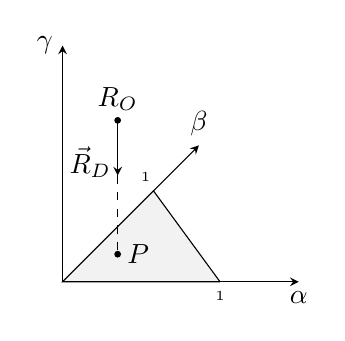
\begin{tikzpicture}
		\coordinate (O) at (0,0,0);
		\def\axisl{3}
		\draw[-stealth] (O) -- (\axisl,0,0) node[below]{$\alpha$};
		\draw[-stealth] (O) -- ({sqrt(\axisl)},{sqrt(\axisl)},0) node[above]{$\beta$};
		\draw[-stealth] (O) -- (0,\axisl,0) node[left]{$\gamma$};
		\coordinate [label={[below,font=\tiny]:$1$}] (V1) at ({\axisl/1.5},0,0);
		\coordinate [label={[shift={(-0.1,0.0)},font=\tiny]:$1$}] (V2) at ({sqrt(\axisl)/1.5},{sqrt(\axisl)/1.5},0);
		\coordinate (V3) at (0,0,0);
		\draw[fill=gray!10] (V1) -- (V2) -- (V3) -- (V1);
		
		\def\xp{0.7};
		\def\yp{0.35};
		\def\xd{0};
		\def\yd{1};
		\def\mag{1.7};
		\coordinate [label=right:$P$] (P) at (\xp,\yp);
		\coordinate [label={[shift={(-0.35,-0.15)}]$\vec{R}_D$}] (RD) at (\xp+\xd,\yp+\yd);
		\coordinate [label=above:$R_O$] (RO) at (\xp+\xd*\mag,\yp+\yd*\mag);
		\draw[fill] (P) circle [radius=1pt];
		\draw[fill] (RO) circle [radius=1pt];
		\draw[-stealth] (RO) -- (RD);
		\draw[dashed] (RD) -- (P);
		\end{tikzpicture}
	\end{subfigure}
	\hfill
\end{figure}
	\begin{equation*}
	R_O + t\vec{R}_D = A+u(B-A)+v(C-A)
	\end{equation*}
	\begin{equation*}
	\begin{bmatrix}
	t \\
	u \\
	v
	\end{bmatrix} 
	= \frac{1}{(D \times E_2) \cdot E_1}
	\begin{bmatrix}
	(T \times E_1) \cdot E_2 \\
	(D \times E_2) \cdot T \\
	(T \times E_1) \cdot D
	\end{bmatrix}
	= \frac{1}{P \cdot E_1}
	\begin{bmatrix}
	Q \cdot E_2 \\
	P \cdot T \\
	Q \cdot D
	\end{bmatrix}
	\end{equation*}
\end{frame}

\begin{frame}[fragile]
	\begin{center}
		\huge{\textbf{La libreria \texttt{TireGround}}}
	\end{center}
\end{frame}

\tikzset{
	treenode/.style = {shape=rectangle, 
		draw, align=center, fill = gray!10},
	root/.style     = {treenode, font=\Large},
	env/.style      = {treenode, font=\ttfamily\normalsize},
	tt/.style      = {font=\ttfamily\normalsize},
	dummy/.style    = {circle,draw}
}

\begin{frame}[fragile]
	\Large{\textbf{\texttt{class Tire}}}
	\normalsize
	\\[0.2cm]
	\begin{figure}[h!]
		\centering
		\begin{tikzpicture}
		[
		grow                    = down,
		sibling distance    = 8em,
		level distance       = 8.5em,
		edge from parent/.style = {draw,-stealth},
		every node/.style       = {font=\footnotesize},
		sloped
		]
		\node [root, env] {Tire}
		child { node [env] {SamplingGrid}
			edge from parent node [below,tt] {Precision} }
		child { node [env] {ETRTO}
			edge from parent node [below,tt] {TireGeometry} }
		child { node [env] {Shadow}
			edge from parent node [below,tt] {TireShadow} }
		child { node [env] {ReferenceFrame}
			edge from parent node [below,tt] {RF} };
		\end{tikzpicture}
	\end{figure}
\end{frame}

\begin{frame}[fragile]
	\Large{\textbf{\texttt{class MagicFormula}}}
	\normalsize
	\\[-1cm]
	\begin{figure}[h!]
		\centering
		\begin{tikzpicture}
		[
		grow                    = down,
		sibling distance    = 8em,
		level distance       = 8.5em,
		edge from parent/.style = {draw,-stealth},
		every node/.style       = {font=\footnotesize},
		sloped
		]
		\node [root, env] {MagicFormula}
		child { node [env] {Tire}
			child { node [env] {SamplingGrid}
				edge from parent node [below,tt] {Precision} }
			child { node [env] {ETRTO}
				edge from parent node [below,tt] {TireGeometry} }
			child { node [env] {Shadow}
				edge from parent node [below,tt] {TireShadow} }
			child { node [env] {ReferenceFrame}
				edge from parent node [below,tt] {RF} }
			edge from parent node [below,tt] {} }
		child { node [env] {Disk}
			edge from parent node [below,tt] {SingleDisk} };
		\end{tikzpicture}
	\end{figure}
\end{frame}

\begin{frame}[fragile]
	\Large{\textbf{\texttt{class MultiDisk}}}
	\normalsize
	\\[-1cm]
	\begin{figure}[h!]
		\centering
		\begin{tikzpicture}
		[
		grow                    = down,
		sibling distance    = 8em,
		level distance       = 8.5em,
		edge from parent/.style = {draw,-stealth},
		every node/.style       = {font=\footnotesize},
		sloped
		]
		\node [root, env] {MultiDisk}
		child { node [env] {Tire}
			child { node [env] {SamplingGrid}
				edge from parent node [below,tt] {Precision} }
			child { node [env] {ETRTO}
				edge from parent node [below,tt] {TireGeometry} }
			child { node [env] {Shadow}
				edge from parent node [below,tt] {TireShadow} }
			child { node [env] {ReferenceFrame}
				edge from parent node [below,tt] {RF} }
			edge from parent node [below,tt] {} }
		child { node [env] {Disk}
			edge from parent node [below,tt] {DiskVec} };
		\end{tikzpicture}
	\end{figure}
\end{frame}

\begin{frame}[fragile]
	\Large{\textbf{Istanziamento della \textit{mesh}}}
\begin{pseudoc}
TireGround::RDF::MeshSurface Road(
    "./file.rdf" // Path to the *.rdf file
);
\end{pseudoc}
\end{frame}	

\begin{frame}[fragile]
	\Large{\textbf{Istanziamento dello pneumatico}}
	\normalsize
\begin{pseudoc}
TireGround::Tire* TireSD = new TireGround::MagicFormula(
    SectionWidth, // [m]
    AspectRatio,  // [%]
    RimDiameter,  // [in]
    SwitchNumber  // Max triangles in the shadow
);
\end{pseudoc}
\begin{pseudoc}
TireGround::Tire* TireMD = new TireGround::MultiDisk(
    SectionWidth, // [m]
    AspectRatio,  // [%]
    RimDiameter,  // [in]
    RadiusVec,    // Disks radius vector [m]
    PointsNumber, // Sampling points for each disk
    SwitchNumber  // Max triangles in the shadow
);
\end{pseudoc}
\end{frame}

\begin{frame}[fragile]
	\Large{\textbf{Posizionamento dello pneumatico nella libreria}}
	\normalsize
\begin{pseudoc}
bool Out = SampleTire->setup(
    Road, // Superficie stradale
    TM    // Matrice di trasformazione 4x4
);
\end{pseudoc}
\begin{pseudoc}
bool Out = SampleTire->setup(
    Normal,   // Vettore normale al piano
    Point,    // Punto appartenente al piano
    Friction, // Coefficiente di attrito nel piano
    TM        // Matrice di trasformazione 4x4
);
\end{pseudoc}
\end{frame}

\begin{frame}[fragile]
	\Large{\textbf{Estrazione dei risultati}}
	\normalsize
\begin{pseudoc}
TireGround::vec3 N;
TireGround::vec3 P;
TireGround::real_type Friction;
TireGround::real_type Rho;
TireGround::real_type RhoDot;
TireGround::real_type RelativeCamber;
TireGround::real_type Area;
TireGround::real_type Volume;

SampleTire->getNormal(N);
SampleTire->getMFpoint(P);
SampleTire->getFriction(Friction);
SampleTire->getRho(Rho);
SampleTire->getRhoDot(PreviousRho,TimeStep,RhoDot);
SampleTire->getRelativeCamber(RelativeCamber);
SampleTire->getArea(Area);
SampleTire->getVolume(Volume);
\end{pseudoc}
\end{frame}

\end{document}